\section*{Review}
\subsection*{}


\textbf{Question 8.} Does the function $f(x,y) = x^2 - y^2$ have a global maximum or minimum?
\begin{respuesta}

\textbf{1.}Draw a direction field for the given differential equation.
\begin{figure}[H]
    \centering
    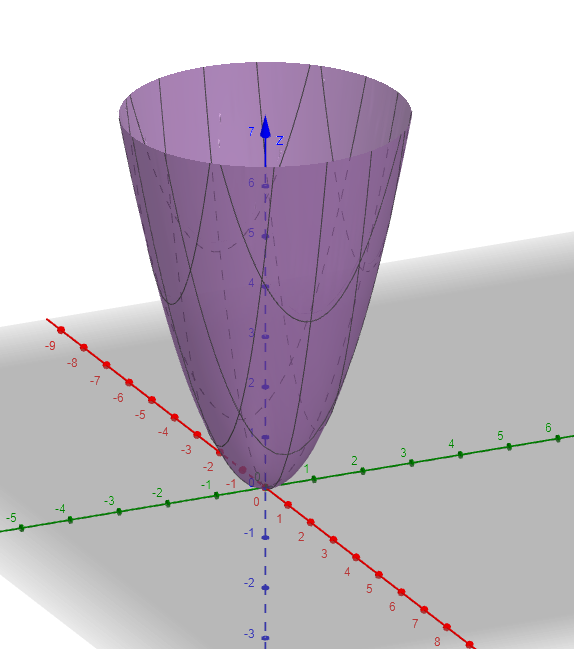
\includegraphics[width=0.5\textwidth]{secciones/michael/images/x_y_graphic.png}
    \caption{Graphic of the function to analyze}
    \label{fig:dirfield}
\end{figure}



\textbf{Checking for Global Maximum:} Fix $y = 0$. Then:
\[
f(x,0) = x^2 \to +\infty \quad \text{as } x \to +\infty
\]
So $f$ is unbounded above $\Rightarrow$ \textbf{no global maximum}.

\medskip
\textbf{Checking for Global Minimum:} Fix $x = 0$. Then:
\[
f(0,y) = -y^2 \to -\infty \quad \text{as } y \to +\infty
\]
So $f$ is unbounded below $\Rightarrow$ \textbf{no global minimum}.

\medskip
\textbf{Critical Point Analysis:} Setting the partial derivatives equal to zero:
\[
\frac{\partial f}{\partial x} = 2x = 0 \implies x = 0, \qquad
\frac{\partial f}{\partial y} = -2y = 0 \implies y = 0
\]
The only critical point is $(0,0)$. Applying the second derivative test:
\[
D = f_{xx}\,f_{yy} - (f_{xy})^2 = (2)(-2) - 0 = -4 < 0
\]
Since $D < 0$, the point $(0,0)$ is a \textbf{saddle point}, not a local extremum.

\textbf{Final answer:}
    \begin{center}
        \fbox{\parbox{0.8\linewidth}{\centering
            The function $f(x,y) = x^2 - y^2$ has \textbf{no global maximum}
            and \textbf{no global minimum}. The unique critical point $(0,0)$
            is a saddle point.
        }}
    \end{center}
\end{respuesta}







\textbf{Question 9.} Let $f(x,y) = xy$, $c(t) = (e^t, \cos(t))$ and $r(t) = f(c(t))$; compute and interpret $dr/dt$.
\begin{respuesta}

First, we find $r(t)$ explicitly:
$$r(t) = f(c(t)) = f(e^t, \cos(t)) = e^t \cos(t)$$

To compute $\frac{dr}{dt}$, we apply the \textbf{Chain Rule}:
$$\frac{dr}{dt} = \frac{\partial f}{\partial x}\frac{dx}{dt} + \frac{\partial f}{\partial y}\frac{dy}{dt}$$

We compute each part:
\begin{itemize}
    \item $\frac{\partial f}{\partial x} = y = \cos(t)$
    \item $\frac{\partial f}{\partial y} = x = e^t$
    \item $\frac{dx}{dt} = \frac{d}{dt}(e^t) = e^t$
    \item $\frac{dy}{dt} = \frac{d}{dt}(\cos(t)) = -\sin(t)$
\end{itemize}

Therefore:
$$\frac{dr}{dt} = \cos(t) \cdot e^t + e^t \cdot (-\sin(t)) = e^t\cos(t) - e^t\sin(t) = e^t(\cos(t) - \sin(t))$$

\textbf{Interpretation:} $\frac{dr}{dt}$ represents the instantaneous rate of change of the composite function $r(t) = e^t\cos(t)$ with respect to $t$. It measures how fast the product $f(x,y) = xy$ changes as the point $(x,y)$ moves along the curve $c(t) = (e^t, \cos(t))$ in the $xy$-plane.

    \textbf{Final answer:}
    \begin{center}
        \fbox{\parbox{0.8\linewidth}{\centering
            $$\frac{dr}{dt} = e^t(\cos(t) - \sin(t))$$
        }}
    \end{center}
\end{respuesta}






\textbf{Question 10.} What is a direction field of a first-order ODE and what is its significance?
\begin{respuesta}

\textbf{Definition:} Consider a first-order ODE of the form:
\[
\frac{dy}{dx} = f(x,y)
\]
A \textbf{direction field} (or \textit{slope field}) is a graphical representation 
constructed by drawing a short line segment at each point $(x,y)$ in the plane 
with slope equal to $f(x,y)$.

\medskip
\textbf{Construction:} At each sampled point $(x_0, y_0)$, we evaluate $f(x_0,y_0)$ 
and draw a small segment with that slope:
\[
\text{slope at } (x_0,\, y_0) \;=\; f(x_0,\, y_0)
\]
Repeating this over a grid of points produces the full direction field.

\medskip
\textbf{Significance:}
\begin{itemize}
    \item \textbf{Qualitative analysis:} It allows us to visualize the behavior 
    of solutions without solving the ODE explicitly.
    \item \textbf{Solution curves:} Any particular solution $y=y(x)$ must be 
    tangent to the direction field at every point it passes through.
    \item \textbf{Equilibria:} Horizontal segments (where $f(x,y)=0$) reveal 
    equilibrium solutions and their stability.
    \item \textbf{No analytic solution needed:} It is especially useful when 
    the ODE has no closed-form solution.
\end{itemize}

    \textbf{Final answer:}
    \begin{center}
        \fbox{\parbox{0.8\linewidth}{\centering
            A direction field of $y' = f(x,y)$ is a plot of short line segments 
            at points $(x,y)$ each with slope $f(x,y)$. Its significance is that 
            it provides a geometric picture of all solutions: solution curves flow 
            tangentially along the segments, revealing behavior, equilibria, and 
            stability without requiring an explicit solution.
        }}
    \end{center}
\end{respuesta}










\textbf{Question 11.} Let $f(x,y) = (x^2 + y^2)\ln(\sqrt{x^2 + y^2})$, $c(t) = (e^t, e^{-t})$ and $r(t) = f(c(t))$; compute and interpret $dr/dt$.
\begin{respuesta}

First, we find $r(t)$ explicitly by substituting $c(t) = (e^t, e^{-t})$ into $f$:
$$r(t) = f(e^t, e^{-t}) = (e^{2t} + e^{-2t})\ln\!\left(\sqrt{e^{2t} + e^{-2t}}\right)$$

Since $\ln(\sqrt{u}) = \frac{1}{2}\ln(u)$, we simplify:
$$r(t) = \frac{1}{2}(e^{2t} + e^{-2t})\ln(e^{2t} + e^{-2t})$$

We apply the \textbf{Chain Rule}:
$$\frac{dr}{dt} = \frac{\partial f}{\partial x}\frac{dx}{dt} + \frac{\partial f}{\partial y}\frac{dy}{dt}$$

\textbf{Computing the partial derivatives of $f$:}

Let $u = x^2 + y^2$, so $f = u \ln(\sqrt{u}) = \frac{1}{2}u\ln(u)$.

$$\frac{\partial f}{\partial x} = \frac{1}{2}\left(\ln(u) \cdot 2x + u \cdot \frac{2x}{u}\right) = x\ln(x^2+y^2) + x = x\left(\ln(x^2+y^2) + 1\right)$$

$$\frac{\partial f}{\partial y} = \frac{1}{2}\left(\ln(u) \cdot 2y + u \cdot \frac{2y}{u}\right) = y\ln(x^2+y^2) + y = y\left(\ln(x^2+y^2) + 1\right)$$

\textbf{Computing the derivatives of the components of $c(t)$:}
$$\frac{dx}{dt} = e^t, \qquad \frac{dy}{dt} = -e^{-t}$$

\textbf{Evaluating at $c(t) = (e^t, e^{-t})$:}
$$\frac{\partial f}{\partial x}\bigg|_{c(t)} = e^t\left(\ln(e^{2t}+e^{-2t})+1\right), \qquad \frac{\partial f}{\partial y}\bigg|_{c(t)} = e^{-t}\left(\ln(e^{2t}+e^{-2t})+1\right)$$

\textbf{Applying the chain rule:}
\begin{align*}
\frac{dr}{dt} &= e^t\!\left(\ln(e^{2t}+e^{-2t})+1\right)\cdot e^t + e^{-t}\!\left(\ln(e^{2t}+e^{-2t})+1\right)\cdot(-e^{-t})\\
&= e^{2t}\!\left(\ln(e^{2t}+e^{-2t})+1\right) - e^{-2t}\!\left(\ln(e^{2t}+e^{-2t})+1\right)\\
&= \left(e^{2t}-e^{-2t}\right)\!\left(\ln(e^{2t}+e^{-2t})+1\right)
\end{align*}

\textbf{Interpretation:} $\frac{dr}{dt}$ represents the instantaneous rate of change of $f$ as the point $(x,y)$ moves along the curve $c(t)=(e^t,e^{-t})$. It combines how sensitive $f$ is to changes in each variable (via $\nabla f$) with how fast the curve moves in each direction (via $c'(t)$). When $t>0$ we have $e^{2t}>e^{-2t}$, so $r(t)$ is increasing; when $t<0$ it is decreasing; and at $t=0$ the rate is zero.

    \textbf{Final answer:}
    \begin{center}
        \fbox{\parbox{0.8\linewidth}{\centering
            $$\frac{dr}{dt} = \left(e^{2t}-e^{-2t}\right)\!\left(\ln(e^{2t}+e^{-2t})+1\right)$$
        }}
    \end{center}
\end{respuesta}






\textbf{Question 12.} What are the solution curves of an ordinary differential equation?
\begin{respuesta}

An \textbf{ordinary differential equation (ODE)} is an equation relating a function of one variable to its derivatives. A \textbf{solution} to an ODE is a function that satisfies the equation on some interval.

\textbf{Solution curves} are the geometric representation of these solutions in the plane. More precisely:

Given an ODE of the form $\frac{dy}{dx} = F(x, y)$, a solution curve is the graph
$$\{(x, y(x)) : x \in I\}$$
of a function $y = y(x)$ defined on some interval $I \subseteq \mathbb{R}$ that satisfies the equation That is at every point $(x_0, y_0)$ on the curve, the slope of the tangent line equals $F(x_0, y_0)$.

\textbf{Key observations:}
\begin{itemize}
    \item The general solution of an ODE contains a family of solution curves, typically parameterized by a constant $C$. Each value of $C$ gives a distinct curve in the $xy$-plane.
    \item A \textbf{particular solution} (obtained by imposing an initial condition $y(x_0) = y_0$) selects exactly oe curve from this family — the unique one passing through $(x_0, y_0)$.
    \item By the existence and uniqueness theorem, solution curves \textbf{do not intersect}, since through each point in the plane there passes at most one solution curve.
    \item The collection of all solution curves is called the \textbf{general solution} and can be visuaized using a \textbf{direction field} (or slope field) where small arrows at each point $(x,y)$ indicate the slope $F(x,y)$ that any solution curve must have there.
\end{itemize}

    \textbf{Final answer:}
    \begin{center}
        \fbox{\parbox{0.8\linewidth}{\centering
            Solution curves of an ODE $\frac{dy}{dx} = F(x,y)$ are the graphs of all functions $y = y(x)$ satisfying the equation. They form a family of non-intersecting curves in the $xy$-plane, each corresponding to a particular value of the integration constant $C$. Imposing an initial condition $y(x_0) = y_0$ selects the unique solution curve passing through the point $(x_0, y_0)$.
        }}
    \end{center}
\end{respuesta}







\textbf{Question 13.} What is the slope of the tangent line to the solution of the 
following differential equation $\dfrac{dy}{dt} = t^2 + y^2$, when it passes through 
the point a.: $(1,2)$; b.: $(0,0)$; c.: $(\pi, e)$; are the solutions of this equation 
always decreasing?
\begin{respuesta}

\textbf{Process:}

The slope of the tangent line at any point $(t, y)$ is given directly by evaluating 
the right-hand side of the ODE at that point.

\textbf{a.} At $(1, 2)$:
\[
    \frac{dy}{dt}\bigg|_{(1,2)} = 1^2 + 2^2 = 1 + 4 = 5
\]

\textbf{b.} At $(0, 0)$:
\[
    \frac{dy}{dt}\bigg|_{(0,0)} = 0^2 + 0^2 = 0
\]

\textbf{c.} At $(\pi, e)$:
\[
    \frac{dy}{dt}\bigg|_{(\pi,\, e)} = \pi^2 + e^2 \approx 9.87 + 7.39 \approx 17.26
\]

\textbf{Decreasing?} Since $t^2 \geq 0$ and $y^2 \geq 0$ for all real $t, y$, we have
$\dfrac{dy}{dt} = t^2 + y^2 \geq 0$ everywhere, with equality only at $(0,0)$.
Therefore, the solutions are \textbf{never decreasing}; they are always non-decreasing 
(strictly increasing except momentarily at the origin).

    \textbf{Final answer:}
    \begin{center}
        \fbox{\parbox{0.8\linewidth}{\centering
            a.\ Slope $= 5$ \quad
            b.\ Slope $= 0$ \quad
            c.\ Slope $= \pi^2 + e^2 \approx 17.26$\\[6pt]
            The solutions are \textbf{never decreasing}, since 
            $t^2 + y^2 \geq 0$ for all $(t,y)$.
        }}
    \end{center}
\end{respuesta}








\textbf{Question 14.} Suppose that $y(x)$ is a function defined implicitly by 
$G(x, y(x)) = k$, where $k$ is a constant and $G$ is a function from $\mathbb{R}^2$ 
to $\mathbb{R}$. If $y(x)$ is differentiable, verify that: 
$\partial G/\partial x + (\partial G/\partial y)(dy/dx) = 0$.
\begin{respuesta}

\textbf{Process:}

Since $k$ is a constant, we differentiate both sides with respect to $x$:
\[
    \frac{d}{dx}\bigl[G(x,\,y(x))\bigr] = \frac{d}{dx}[k] = 0.
\]
The left-hand side involves a composition: $G$ depends on $x$ directly 
and also through $y(x)$. Applying the \textbf{multivariable Chain Rule}:
\[
    \frac{d}{dx}\bigl[G(x,\,y(x))\bigr]
    = \frac{\partial G}{\partial x}\cdot\underbrace{\frac{dx}{dx}}_{=\,1}
    + \frac{\partial G}{\partial y}\cdot\frac{dy}{dx}.
\]
Therefore, setting this equal to zero:
\[
    \frac{\partial G}{\partial x} + \frac{\partial G}{\partial y}\,\frac{dy}{dx} 
    = 0.  
\]
Moreover, solving for $dy/dx$ (provided $\partial G/\partial y \neq 0$) 
recovers the \textbf{Implicit Function Theorem} formula:
\[
    \frac{dy}{dx} = -\frac{\,\partial G/\partial x\,}{\partial G/\partial y}.
\]

    \textbf{Final answer:}
    \begin{center}
        \fbox{\parbox{0.8\linewidth}{\centering
            Differentiating both sides of $G(x,y(x))=k$ with respect 
            to $x$ and applying the multivariable Chain Rule:
            \[
                \frac{d}{dx}\bigl[G(x,y(x))\bigr]
                = \frac{\partial G}{\partial x}
                + \frac{\partial G}{\partial y}\,\frac{dy}{dx}
                = \frac{d}{dx}[k] = 0 \qquad \blacksquare
            \]
        }}
    \end{center}
\end{respuesta}